\section{Erläuterungen zu OPPs und der Kretschmann-\\Konfiguration}\label{sec:erläuterung}
\footnote[1]{In diesem Versuchsbericht werden häufig die physikalischen Hintergründe zu OPPs und den verwendeten Messverfahren erläutert.
Um die Übersichtlichkeit zu wahren, werden häufig bei einigen Erklärungen nicht die genauen Literaturverweise angegeben. Die Informationen sind stets
\cite{linden_optik}, \cite{linden_photonics}, \cite{nano}, \cite{prism}, \cite{wiki:sp}, \cite{wiki:spp} und \cite{wiki:spr} entnommen. An notwendigen Stellen
werden diese dennoch explizit angegeben.}Bei der Auswertung und Analyse dieses Versuches ist ein grundlegendes Verständnis zu OPPs und der Kretschmann-Konfiguration notwendig.
Aus diesem Grund werden hier einige der zentralen Konzepte erläutert, sodass sich bei der Auswertung und Analyse des Versuches
darauf bezogen werden kann.\par
Die Amplituden der elektromagnetischen Felder des sichtbaren Lichtes fallen in Metallen exponentiell ab (näheres dazu ist in \cite{linden_optik} und \cite{linden_photonics}
zu finden). Dennoch können an der Grenzfläche zwischen einem Metall und einem Dielektrikum Oberflächenwellen (OPPs) existieren. Diese stellen
einen Mischzustand aus einer elektromagnetischen Welle und einer longitudinalen Elektronendichtewelle dar.\par
Im Folgenden wird Licht der Frequenz $\omega$ betrachtet. Dieses treffe mit einem Einfallswinkel $\theta$ (gemessen zwischen dem Wellenvektor des einlaufenden Lichtes
und der Normalen der Grenzfläche) von einem Dielektrikum kommend auf eine Dielektrikum-Metall-Grenzfläche. Dieses System befinde sich in Luft. Das einlaufende Licht wird teilweise reflektiert und teilweise transmittiert.
Der Wellenvektor der transmittierten Welle $\vec{k}_{\mathrm{t}}$ lässt sich zu $\vec{k}_{\mathrm{t},\parallel} + \vec{k}_{\mathrm{t},\perp}$ zerlegen, wobei
$\vec{k}_{\mathrm{t},\parallel}$ der Anteil des Wellenvektors des transmittierten Lichtes parallel und $\vec{k}_{\mathrm{t},\perp}$ der Anteil des
Wellenvektors des transmittierten Lichtes senkrecht zur Grenzfläche ist. Mithilfe dessen wird in \cite{linden_optik} demonstriert, dass sich die transmittierte elektromagnetische
Welle entlang der Dielektrikum-Metall-Grenzfläche ausbreitet und die zugehörige Amplitude senkrecht zu der Dielektrikum-Metall-Grenzfläche exponentiell im Metall
abfällt. Ist die Metallschicht dünn genug (für die meisten Metalla nicht dicker als \SI{100}{\nm}), so reicht die Amplitude der transmittierten elektromagnetischen
Welle bis zu der Metall-Luft-Grenzfläche. Dann können an dieser Grenzfläche OPPs angeregt werden, da die Metallschicht viele freie Ladungsträger hat, welche
durch die transmittierte elektromagnetische Welle zu einer longitudinalen Elektronendichtewelle angeregt werden. Da die freien Ladungsträger dabei oszillieren, wird
eine elektromagnetische Welle abgestrahlt. Diese propagiert entlang der Metall-Luft-Grenzfläche und fällt in beiden Medien exponentiell ab. Dabei ist der exponentielle
Abfall in Metall stärker als in Luft, da die Licht sehr stark mit den freien Ladungsträgern des Metalls wechselwirkt und daher stärker absorbiert wird.
Die resultierende elektromagnetische Feldverteilung der OPPs ist in \cref{fig:feldverteilung} gezeigt. Eine sehr ausführliche Diskussion zu OPPs ist in \cite{nano} zu finden.
\begin{figure}[H]
    \centering
    \begin{subfigure}{0.4\textwidth}
        \centering
        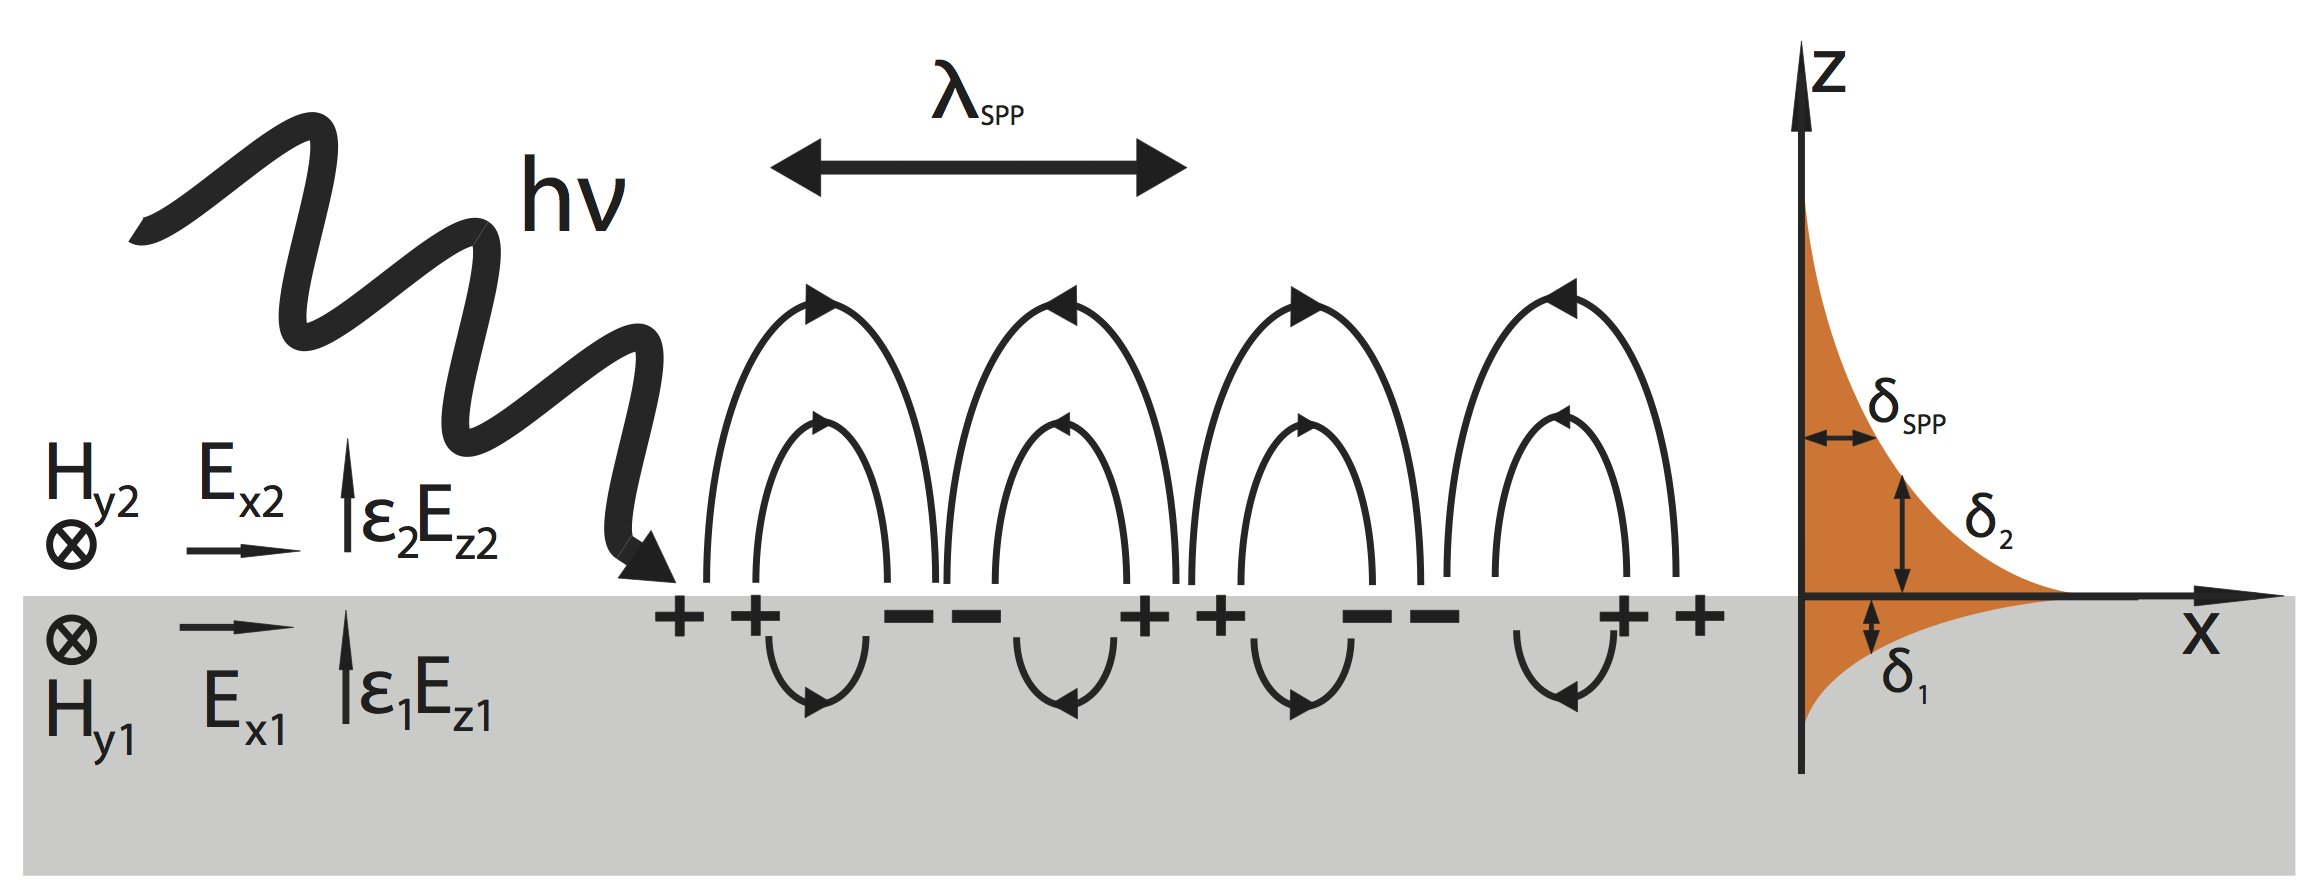
\includegraphics[width=\linewidth]{../figs/Sketch_of_surface_plasmon}
        \caption{\cite{wiki:sp}}
    \end{subfigure}
    \begin{subfigure}{0.4\textwidth}
        \centering
        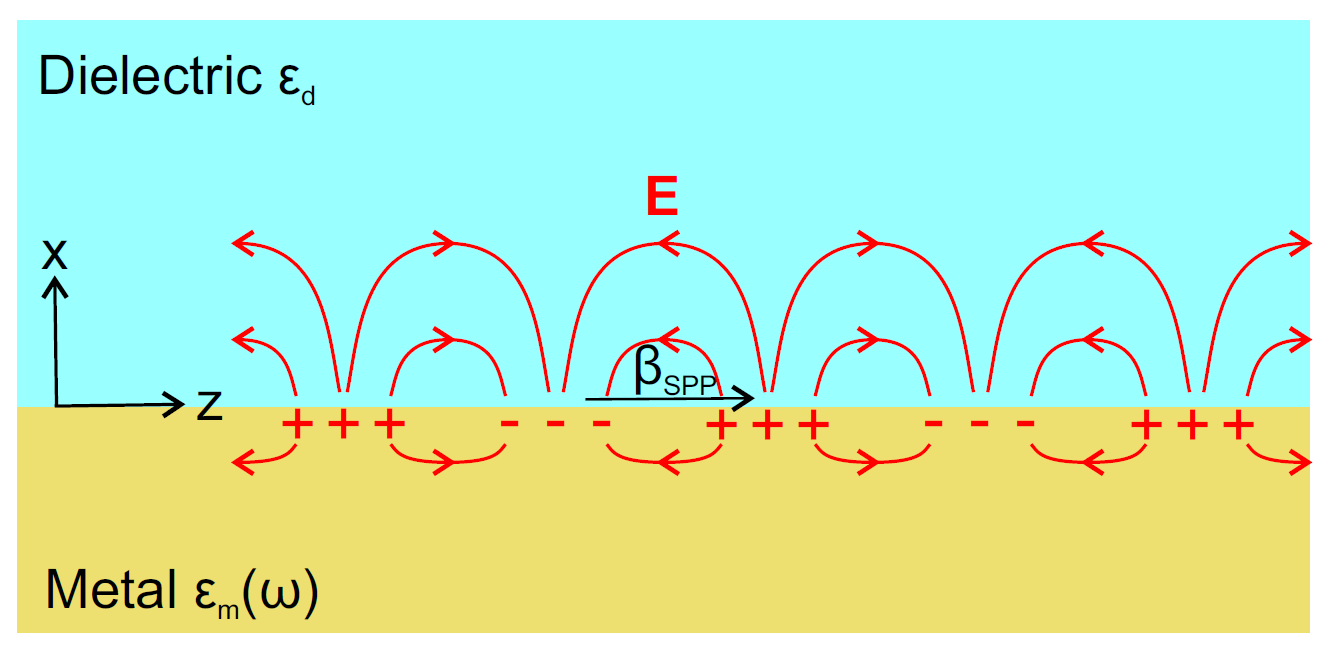
\includegraphics[width=\linewidth]{../figs/field_scheme}
        \caption{\cite{linden_photonics}}
    \end{subfigure}
    \caption{Elektromagnetische Feldverteilung von OPPs an einer Metall-Luft-Grenzfläche.}\label{fig:feldverteilung}
\end{figure}
OPPs können nur unter bestimmten Bedingungen angeregt werden. In \cite{nano} wird gezeigt, dass nur OPPs existieren, dessen elektromagnetisches Feld eine TM-Polarisation (magnetisches Feld
parallel zu Grenzfläche) bzw. p-Polarisation (elektrisches Feld parallel zur Einfallsebene). Es existieren keine TE-Moden (elektrisches Feld parallel zur Grenzfläche).
Dies kann durch Lösen der Maxwell-Gleichungen gezeigt werden. Demnach können OPPs zu angeregt werden, wenn das einfallende Licht TM- bzw- p-polarisiert ist. Für
TE- bzw- s-polarisation wird erwartet, dass das Licht nahezu vollständig reflektiert wird, da es nahezu keinen Energie- und Impulsübertrag gibt, durch den OPPs
angeregt werden können. Allgemein falls keine OPPs angeregt werden, wird das Licht nur nahezu vollständig reflektiert (Reflexionsgrad $R \approx 1$), was ein typisches
Verhalten von Metall (siehe \cite{linden_optik}) ist. In dem Versuch wird stets die reflektierte Intensität gemessen. Mit dieser lässt sich der Reflexionsgrad bestimmen.
Wenn im Versuch OPPs angeregt werden, wird ein Minimum des Reflexionsgrades erwartet, da dann das Licht zur Anregung der OPPs absorbiert wird.\par
Eine weitere Bedingung zur Anregung von OPPs wird durch die Dispersionsrelation vorgegeben. Die Disperionsrelation von OPPs ist nach \cite{linden_optik} durch
\begin{equation}\label{eq:k_spp}
    k_{\mathrm{SPP}} = \frac{\omega}{c_0} \sqrt{\frac{\epsilon_{\mathrm{d}}\epsilon_{\mathrm{m}}}{\epsilon_{\mathrm{d}} + \epsilon_{\mathrm{m}}}}
\end{equation} gegeben, wobei $c_0$ die Vakuumlichtgeschwindigkeit, $\epsilon_{\mathrm{d}}$ die dielektrische Funktion des Dielektrikums und $\epsilon_{\mathrm{m}}$
die dielektrische Funktion des Metalls ist. Allgemein können mithilfe der dielektrischen Funktion die optischen Eigenschaften eines Mediums beschrieben werden.
Nach \cite{linden_photonics} können OPPs nur dann angeregt werden, wenn der Betrag des zur Grenzfläche parallelen Anteils des Wellenvektors des einfallenden Lichtes
gleich $k_{\mathrm{SPP}}$ ist (Impulserhaltung). Wenn das einfallende Licht aus Luft kommt, muss also
\begin{equation*}
    k_{\mathrm{SPP}} = \frac{\omega}{c_0}\sqrt{\frac{\epsilon_{\mathrm{Luft}}\epsilon_{\mathrm{m}}}{\epsilon_{\mathrm{Luft}} + \epsilon_{\mathrm{m}}}} = \frac{\omega}{c_0}\sqrt{\epsilon_{\mathrm{Luft}}} \sin(\theta) = \frac{\omega}{c_0}n_{\mathrm{Luft}} \sin(\theta)
\end{equation*} gelten. Wegen $\max(\sin(\theta)) = 1$ und den Eigenschaften der dielektrischen Funktion des Metalls $\epsilon_{\mathrm{m}}$ (weitere Informationen
dazu sind in \cite{linden_photonics} und \cite{nano} zu finden), kann diese Bedingung nie erfüllt werden. Es ist also $k_{\mathrm{SPP}} > \frac{\omega}{c_0}\sqrt{\epsilon_{\mathrm{Luft}}}\sin(\theta)$.
Dieser Zusammenhang ist in \cref{fig:dispersion} dargestellt, da sich hier die Dispersionskurve der OPPs nie mit der des Lichtes in Luft schneidet.
\begin{figure}[H]
	\centering
	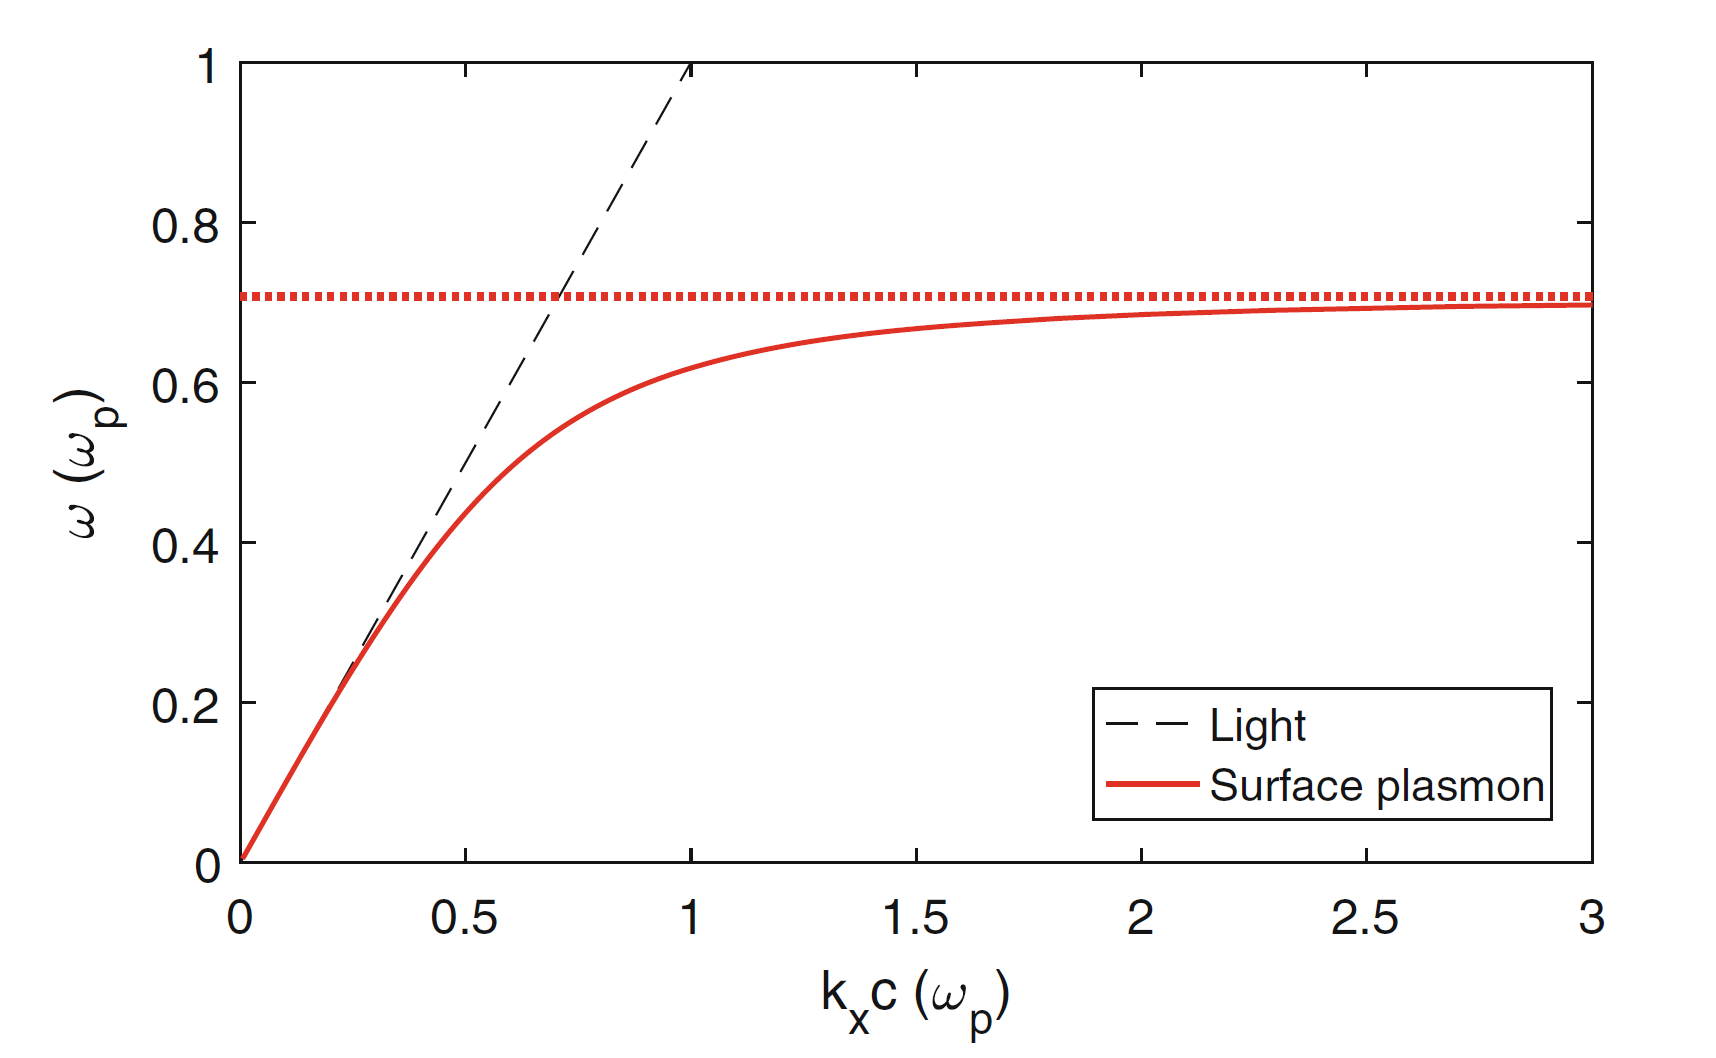
\includegraphics[width=0.6\linewidth]{../figs/dispersion.png}
	\caption{Darstellung der Dispersionsrelation von OPPS und der von Licht (berechnet mit $\epsilon_{\mathrm{Luft}} = 1$ und $\epsilon_{\mathrm{m}} = 1 - \frac{\omega_{\mathrm{p}}^2}{\omega^2}$ (Drude-Modell)) \cite{nano}.}
	\label{fig:dispersion}
\end{figure} Um OPPs mithilfe von Licht anzuregen, wird also ein Dielektrikum mit einem Brechungsindex benötigt, der größer ist als der von Luft. Hier bietet sich zum Beispiel Glas ein.
Eine mögliche experimentelle Umsetzung dieser Idee ist durch die Kretschmann-Konfiguration gegeben (siehe \cref{fig:kretschmann}). Die Bedingung $k_{\mathrm{SPP}} = \frac{\omega}{c_0}n_{\mathrm{Prisma}}\sin(\theta)$
kann nun erreicht werden, womit eine Anregung von OPPs unter einem bestimmten Einfallswinkel möglich ist.
\begin{figure}[H]
	\centering
	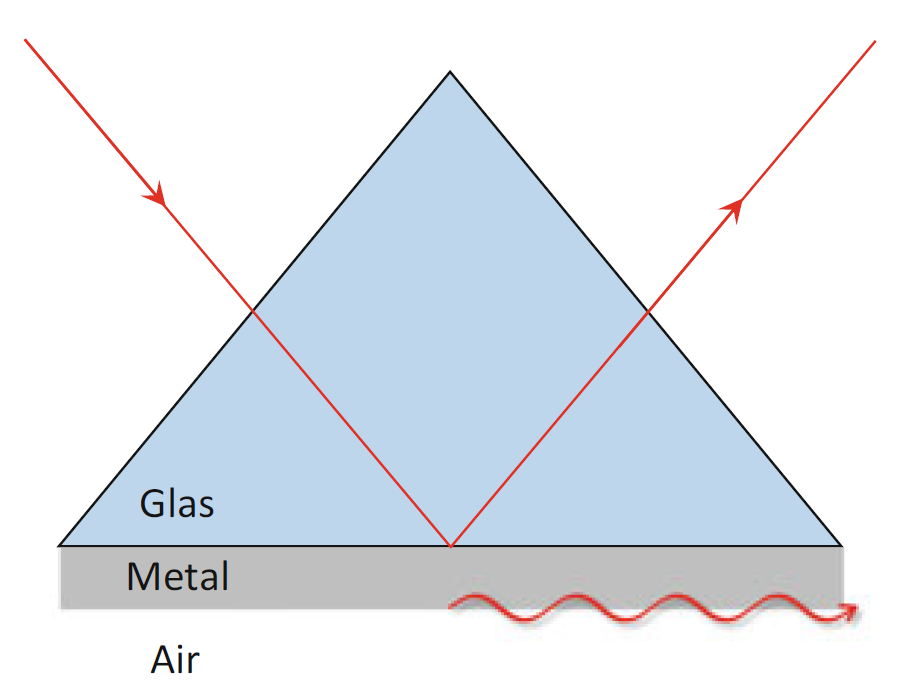
\includegraphics[width=0.4\linewidth]{../figs/kretschmann.png}
	\caption{Kretschmann-Konfiguration zur Anregung von OPPs \cite{nano}.}
	\label{fig:kretschmann}
\end{figure}